\section{Tropical Rainforest} \label{sec:results_trop_rainforest}

Tropical rainforest or equatorial climates are characterised by frequent and heavy rainfall and are situated on or close to the equator. Because of their location they have are no seasons and therefore very little temperature and illumination variance throughout the year.\\

Toamasina, a city in Madagascar at latitude 18\textdegree south, is the location on which climate data is based for these tests.\\

Because of its water absorption capabilities, loamy soil is modelled in this test scenario. To do so, the terrain is filled with a base soil infiltration rate of fifteen millimetres per hour (see table \ref{tab:soil_types} for the correlation between soil type and soil infiltration rate). To model rocky cliff faces, the soil infiltration rate is set to zero when the slope angle surpasses forty degrees.\\

The configured monthly rainfall, rainfall intensity and resulting soil moisture and weighted soil moisture is summarized in table \ref{tab:results_tropical_input_resources}. The resulting water networks that form on the terrain are illustrated in figure \ref{fig:results_tropical_water_networks}.\\

The temperature extremes configured are twenty-one degrees for June and twenty-six degrees for December, resulting in monthly temperatures outlined in table \ref{tab:results_tropical_input_resources}. The lapse rate is kept at its default value of 6.5 degrees loss for every thousand metres gained. \\

\definecolor{green}{rgb}{0,1,0}
\begin{table}[htb!]
  \centering
	    \begin{tabular}{|p{3cm}|p{.7cm}|p{.7cm}|p{.7cm}|p{.7cm}|p{.7cm}|p{.7cm}|p{.7cm}|p{.7cm}|p{.7cm}|p{.7cm}|p{.7cm}|p{.7cm}|}
		\hline	
  	    \textbf{Resource} & \textbf{Jan} & \textbf{Feb} & \textbf{Mar} & \textbf{Apr} & \textbf{May} & \textbf{Jun} & \textbf{Jul} & \textbf{Aug} & \textbf{Sep} & \textbf{Oct} & \textbf{Nov} & \textbf{Dec} \\
  	    \hline	
		Rainfall (mm) & \cellcolor{green}410 & \cellcolor{green}382 & \cellcolor{green}478 & \cellcolor{green}322 & \cellcolor{green}228 & \cellcolor{green}259 & \cellcolor{green}288 & \cellcolor{green}218 & \cellcolor{green}121 & \cellcolor{green}132 & \cellcolor{green}169 & \cellcolor{green}357  \\
		\hline
		Rainfall Intensity (mm/h) & \cellcolor{green}18 & \cellcolor{green}17 & \cellcolor{green}20 & \cellcolor{green}16 & \cellcolor{green}11 & \cellcolor{green}12 & \cellcolor{green}14 & \cellcolor{green}11 & \cellcolor{green}7 & \cellcolor{green}7 & \cellcolor{green}8 & \cellcolor{green}16  \\
		\hline
		Soil Moisture (mm) & 341 & 337 & 359 & 302 & 228 & 259 & 288 & 218 & 121 & 132 & 169 & 334  \\
		\hline
		Weighted soil moisture (mm)	& 311 & 338	& 349 & 327 & 274 & 256 & 268 & 248 & 181 & 143 & 149 & 246 \\
		\hline
		Temperature (\textdegree) & 25 & 24 & 24 & 23 & 22 & \cellcolor{green}21 & 22 & 23 & 24 & 24 & 25 & \cellcolor{green}26  \\
		\hline
		\end{tabular}
		\caption{Tropical rainforest: Monthly rainfall, rainfall intensity, soil moisture, weighted soil moisture and temperature at zero metres. Green cells represent values explicitly input for this test scenario, all others are procedurally calculated. The soil moisture is valid for terrain vertices with a slope less than forty degrees and therefore for which the soil infiltration rate is 15 mm per hour. All other vertices have a soil moisture of zero (modelled rock cliff faces).}
	  \label{tab:results_tropical_input_resources}
\end{table}

\begin{figure}[htb!]
\center
	\includegraphics[width=\textwidth]{results_tropical_water_networks.png}
	\caption{ \textit{Tropical rainforest: Water networks that form on the terrain in every month. From left to right, top to bottom.}}
	\label{fig:results_tropical_water_networks}
\end{figure}

The number of generated clusters is set to ten. The clustered terrain is shown in figure \ref{fig:results_tropical_terrain_clusters} and the corresponding cluster properties summarized in figure \ref{fig:results_tropical_cluster_hum_temp_illum} and table \ref{tab:results_tropical_cluster_slope_covarea}. 

\begin{figure}[htb!]
\center
	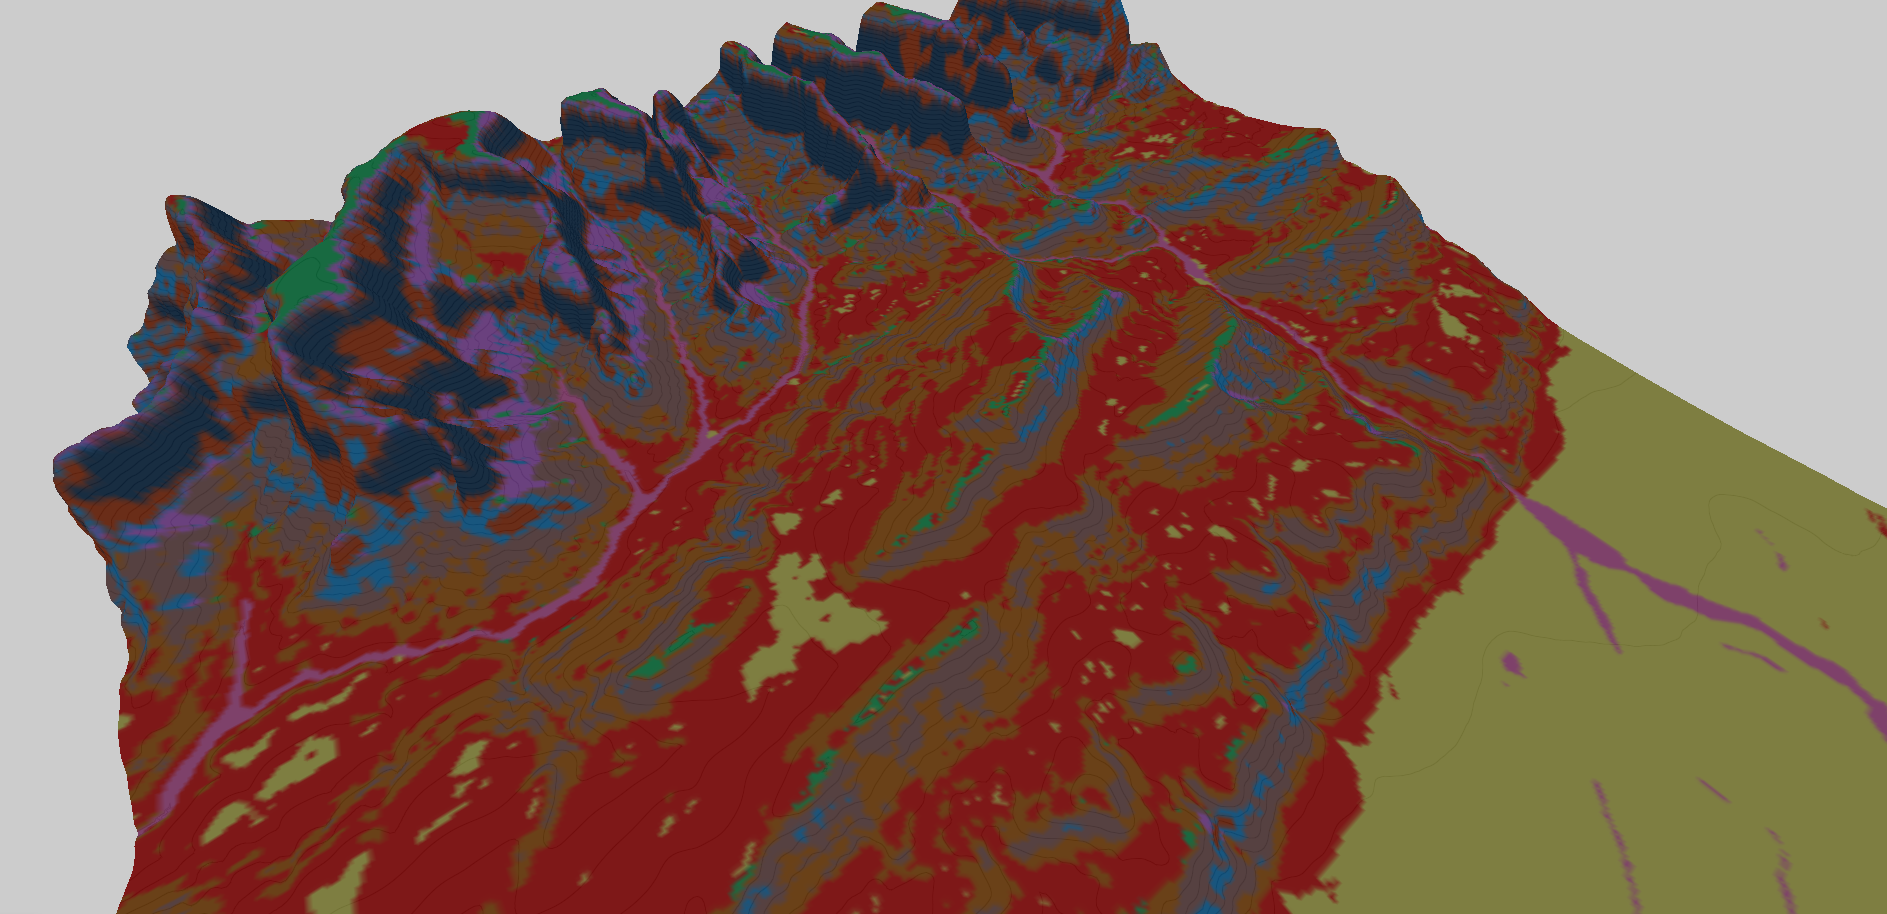
\includegraphics[width=\textwidth]{results_tropical_clusters_on_terrain.png}
	\caption{ \textit{Tropical rainforest: Resulting terrain clusters.} }
	\label{fig:results_tropical_terrain_clusters}
\end{figure}

\begin{figure}[htb!]
\center
	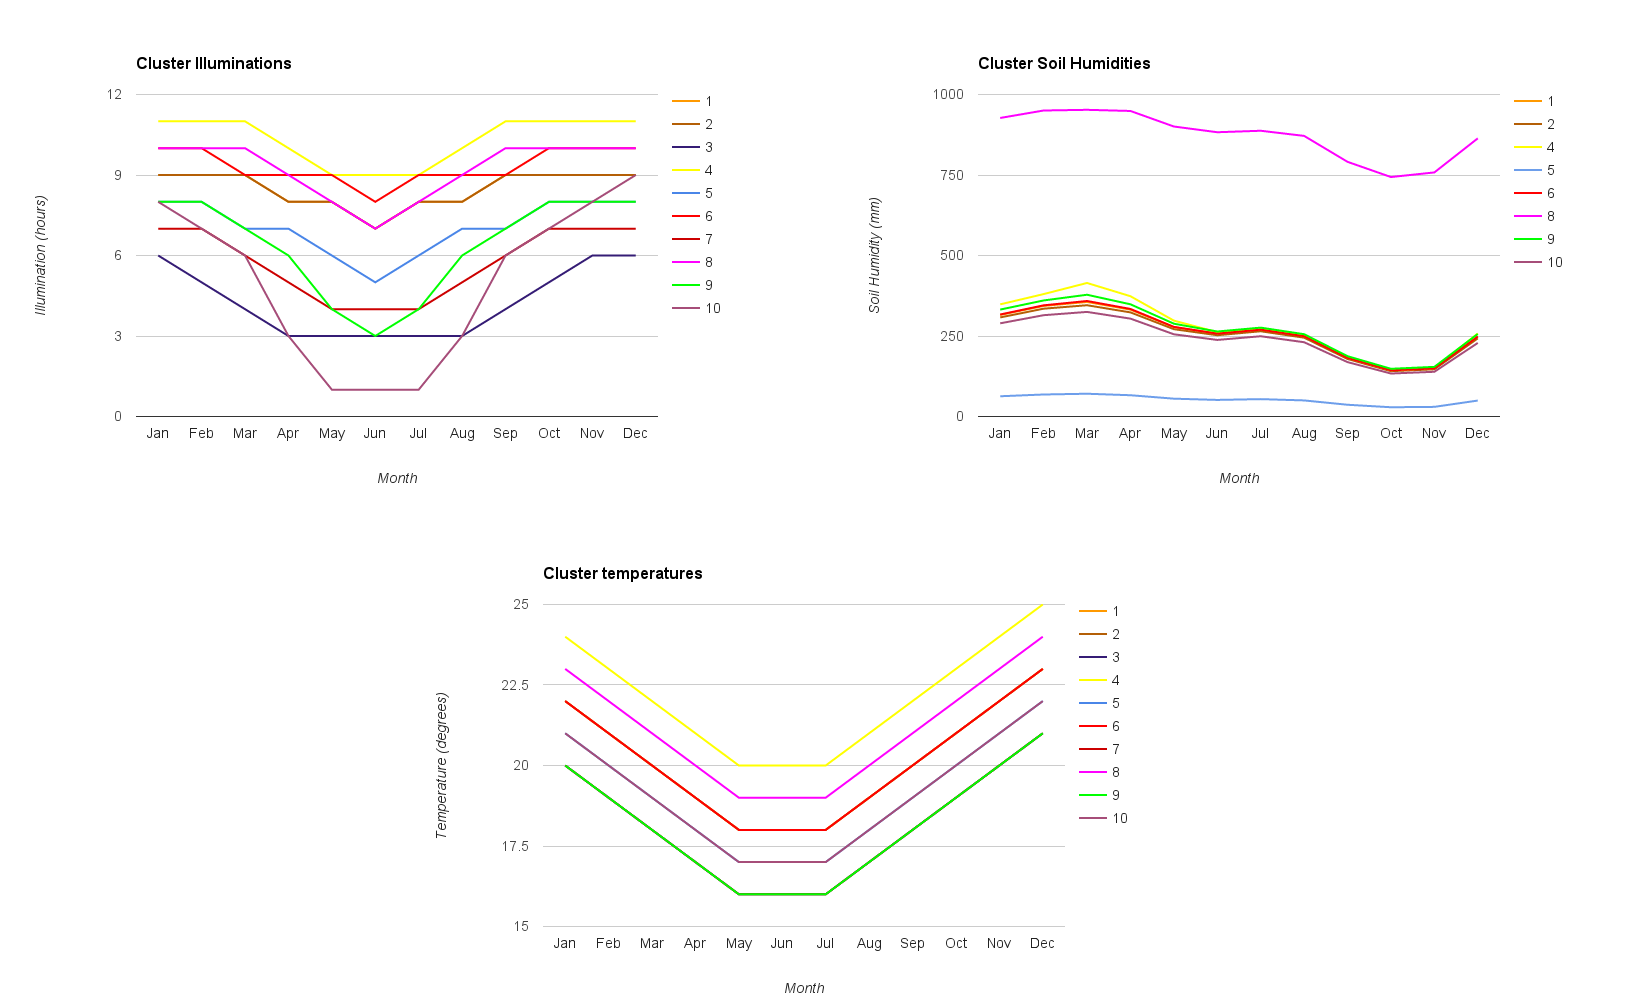
\includegraphics[height=\textheight-60pt,keepaspectratio]{results_tropical_clusters_hum_temp_illum.png}
	\caption{ \textit{Tropical rainforest: Monthly sun exposure (top), temperatures (middle) and soil moistures (bottom) for each terrain cluster. Note that soil humidity data is removed for clusters (3 and 7) as the corresponding values are too small.}}
	\label{fig:results_tropical_cluster_hum_temp_illum}
\end{figure}

\begin{table}[htb!]
  \centering
	    \begin{tabular}{|p{5cm}|p{5cm}|p{5cm}|}
		\hline	
  	    \textbf{Cluster} & \textbf{Slope (degrees)} & \textbf{Coverage area (\% of terrain)} \\
  	    \hline	
		Cluster 1 & 22.3 & 19.3 \\
		\hline
		Cluster 2 & 32.2704 & 16.2 \\
		\hline
		Cluster 3 & 69.092 & 4.7 \\
		\hline
		Cluster 4 & 2.95581 & 18.1 \\
		\hline
		Cluster 5 & 42.9369 & 4.8 \\
		\hline
		Cluster 6 & 11.8319 & 22.1 \\
		\hline
		Cluster 7 & 54.1674 & 6.0 \\
		\hline
		Cluster 8 & 8.0803 & 2.1 \\
		\hline
		Cluster 9 & 14.0102 & 2.5 \\
		\hline
		Cluster 10 & 32.1679 & 3.8 \\
		\hline
		\end{tabular}
		\caption{Tropical rainforest: Slope and coverage area of each cluster.}
	  \label{tab:results_tropical_cluster_slope_covarea}
\end{table}

Five tropical rainforest plant species are configured for this test: \textit{Brazil nut}, \textit{Cavendish banana}, \textit{Heliconia}, \textit{King of Bromeliads} and \textit{Orchid}. The properties associated with each are summarized in appendix \ref{AppendixE}.\\

The species suitability filtering (see section \ref{sec:plant_suitability_filtering}) automatically filters out ill-suited species from being inserted in some clusters as the slope, soil moisture and/or temperature do not meet the requirements of the given species. Note that species are not filtered out due to unsuited illumination during specie suitability filtering as the sun exposure can vary during a simulation as canopy plants grow and project shade. Table \ref{tab:results_tropical_species_suitability} summarizes this information and illustrates the species which are suited to individual clusters and, if not, which resource acts as a bottleneck. From this, it is possible to conclude that no plants are able to grow, and therefore no ecosystem simulator needs to be run, for clusters 3, 5, 7 and 8. Clusters 3, 5 and 7 have to steep a slope and too little soil humidity to cater for these species. \textit{Cluster 8} has soil that is too moist as it represents the points on the terrain with standing water.\\

\definecolor{color_red}{rgb}{1.0,0.0,0.0}
\definecolor{color_green}{rgb}{0.0,1.0,0.0}
\definecolor{color_orange}{rgb}{1.0,0.65,0.0}

\begin{table}[htb!]
  \centering
	    \begin{tabular}{|p{2cm}|p{2.5cm}|p{2.5cm}|p{2.5cm}|p{2.5cm}|p{2.5cm}|}
		\hline	
		&  \textbf{Orchid} & \textbf{Cavendish banana} & \textbf{Heliconia} & \textbf{Brazil Nut} & \textbf{King of Bromeliads}\\
		\hline	
		Cluster 1 & 
		Y & 
		Y & 
		Y & 
		Y & 
		Y \\
		\hline	
		Cluster 2 & 
		Y & 
		\cellcolor{color_red}N (S$^{+}$) & 
		Y & 
		\cellcolor{color_red}N (S$^{+}$) & 
		Y \\
		\hline	
		Cluster 3 & 
		\cellcolor{color_red}N (S$^{+}$, SH$^{-}$) & 
		\cellcolor{color_red}N (S$^{+}$, SH$^{-}$) & 
		\cellcolor{color_red}N (S$^{+}$, SH$^{-}$) & 
		\cellcolor{color_red}N (S$^{-}$, SH$^{-}$) & 
		\cellcolor{color_red}N (S$^{+}$, SH$^{+}$) \\
		\hline	
		Cluster 4 & 
		Y & 
		Y & 
		Y & 
		Y & 
		Y \\
		\hline	
		Cluster 5 & 
		\cellcolor{color_red}N (SH$^{-}$) & 
		\cellcolor{color_red}N (S$^{+}$, SH$^{-}$) & 
		\cellcolor{color_red}N (S$^{+}$, SH$^{-}$) & 
		\cellcolor{color_red}N (S$^{+}$, SH$^{-}$) & 
		\cellcolor{color_red}N (SH$^{-}$) \\
		\hline	
		Cluster 6 & 
		Y & 
		Y & 
		Y & 
		Y &
		Y \\
		\hline	
		Cluster 7 & 
		\cellcolor{color_red}N (SH$^{-}$) &
		\cellcolor{color_red}N (S$^{+}$, SH$^{-}$) &
		\cellcolor{color_red}N (S$^{+}$, SH$^{-}$) & 
		\cellcolor{color_red}N (S$^{+}$, SH$^{-}$) & 
		\cellcolor{color_red}N (S$^{+}$, SH$^{-}$) \\
		\hline	
		Cluster 8 & 
		\cellcolor{color_red}N(SH$^{+}$) & 
		\cellcolor{color_red}N (SH$^{+}$) & 
		\cellcolor{color_red}N (SH$^{+}$) & 
		\cellcolor{color_red}N (SH$^{+}$) & 
		\cellcolor{color_red}N (SH$^{+}$) \\
		\hline	
		Cluster 9 & 
		Y & 
		Y & 
		Y & 
		Y & 
		Y \\
		\hline	
		Cluster 10 &
		Y & 
		\cellcolor{color_red}N (S$^{+}$) & 
		Y & 
		\cellcolor{color_red}N (S$^{+}$) & 
		Y \\
		\hline	
		\end{tabular}
		\caption{Tropical rainforest: Summary of the species suitability filter pass on each cluster. This step filters out ill-suited species from being inserted into a given cluster is the slope, soil humidity or temperature is ill-suited. If a species is not suited, the cell is highlighted red and the reason is stated in brackets where \textit{S} is the slope, \textit{T} is the temperature and \textit{SH} is the soil humidity, $^{+}$ signifies too much and $^{-}$ too little of the given resource.}
	  \label{tab:results_tropical_species_suitability}
\end{table}

Figures \ref{fig:results_tropical_brazil_nut_suitability}, \ref{fig:results_tropical_cavendish_banana_suitability}, \ref{fig:results_tropical_heliconia_suitability}, \ref{fig:results_tropical_king_of_bromeliads_suitability}, \ref{fig:results_tropical_orchid_suitability} and table \ref{tab:results_tropical_species_slope_suitability} illustrate how suited the remaining clusters are for each plant species. This information proves especially useful for determining how suited given species are in terms of illumination, as the species suitability scoring ignores this resource since it varies throughout a simulation as plants grow and project shade.\\
From this, it is possible to conclude that: \textit{Clusters 9 and 10} prevent \textit{Brazil Nut}, \textit{Cavendish Banana} and \textit{Heliconia} from growing as their minimum illuminations falls below these species lower limits. These clusters also prevent shade-loving \textit{King of Bromeliads} and \textit{Orchids} from growing as their maximum illumination surpasses the species upper limits. Clusters 9 and 10 are therefore unsuited to all species.\\
\textit{Cavendish Banana} and \textit{Brazil Nut} plants are unsuited to clusters 1 and 2 as the clusters minimum illumination falls below the species lower limit.\\
\textit{King of Bromeliads} and \textit{Orchids} are universally unsuited as the clusters maximum illuminations surpass the species upper-limit. However, as these species are shade-loving, there is a possibility they survive in the undergrowth of striving plant instances. Given all this, the clusters to which plant species are suited and plausible distributions created are clusters 1, 2, 4 and 6. Together, these clusters make up only 70\% of the terrain.\\

\begin{figure}[htb!]
\center
	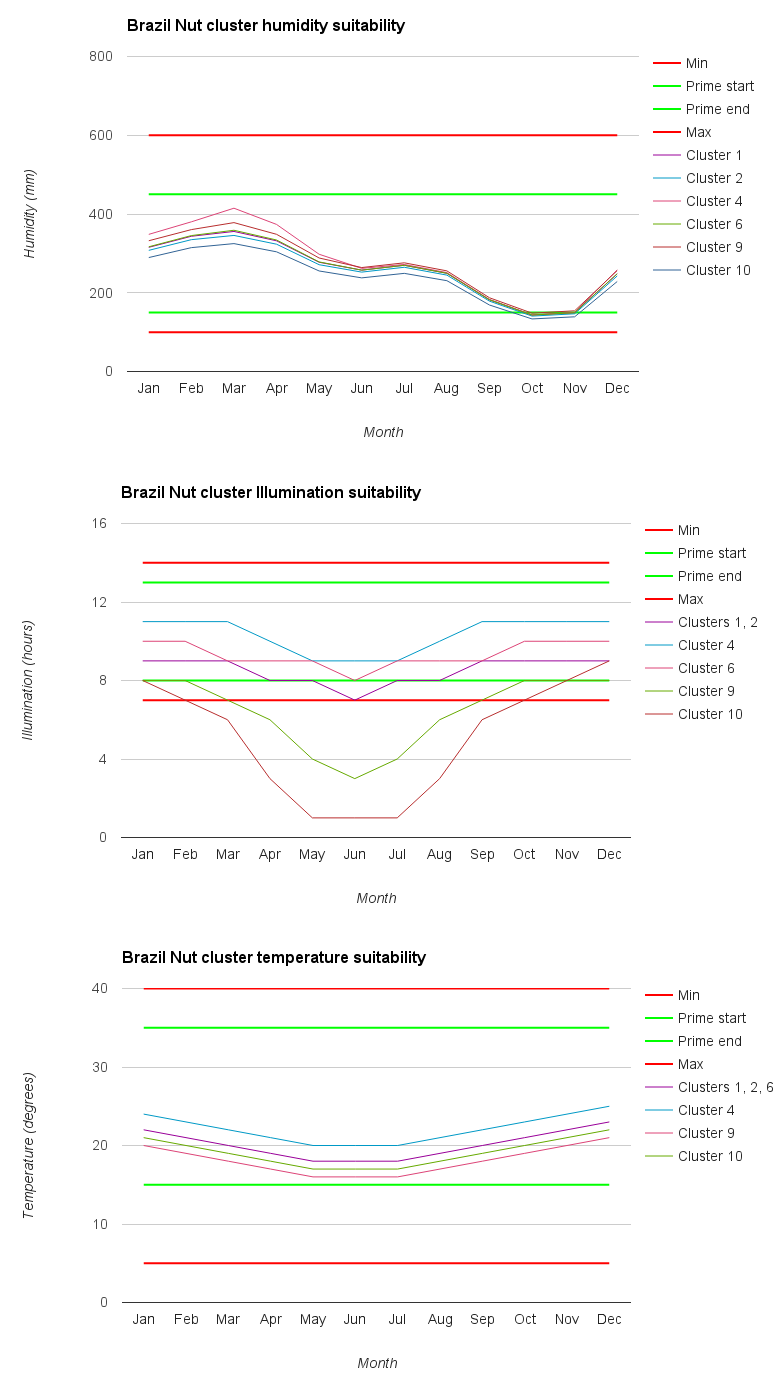
\includegraphics[height=\textheight-100pt,keepaspectratio]{brazil_nut_suitability.png}
	\caption{ \textit{Tropical rainforest: Brazil nut suitability to clusters 1, 2, 4, 6, 9 and 10 in terms of soil moisture (top), illumination (middle) and temperature. The thick green lines and red lines delimit the species prime range and absolute limits, respectively.} }
	\label{fig:results_tropical_brazil_nut_suitability}
\end{figure}

\begin{figure}[htb!]
\center
	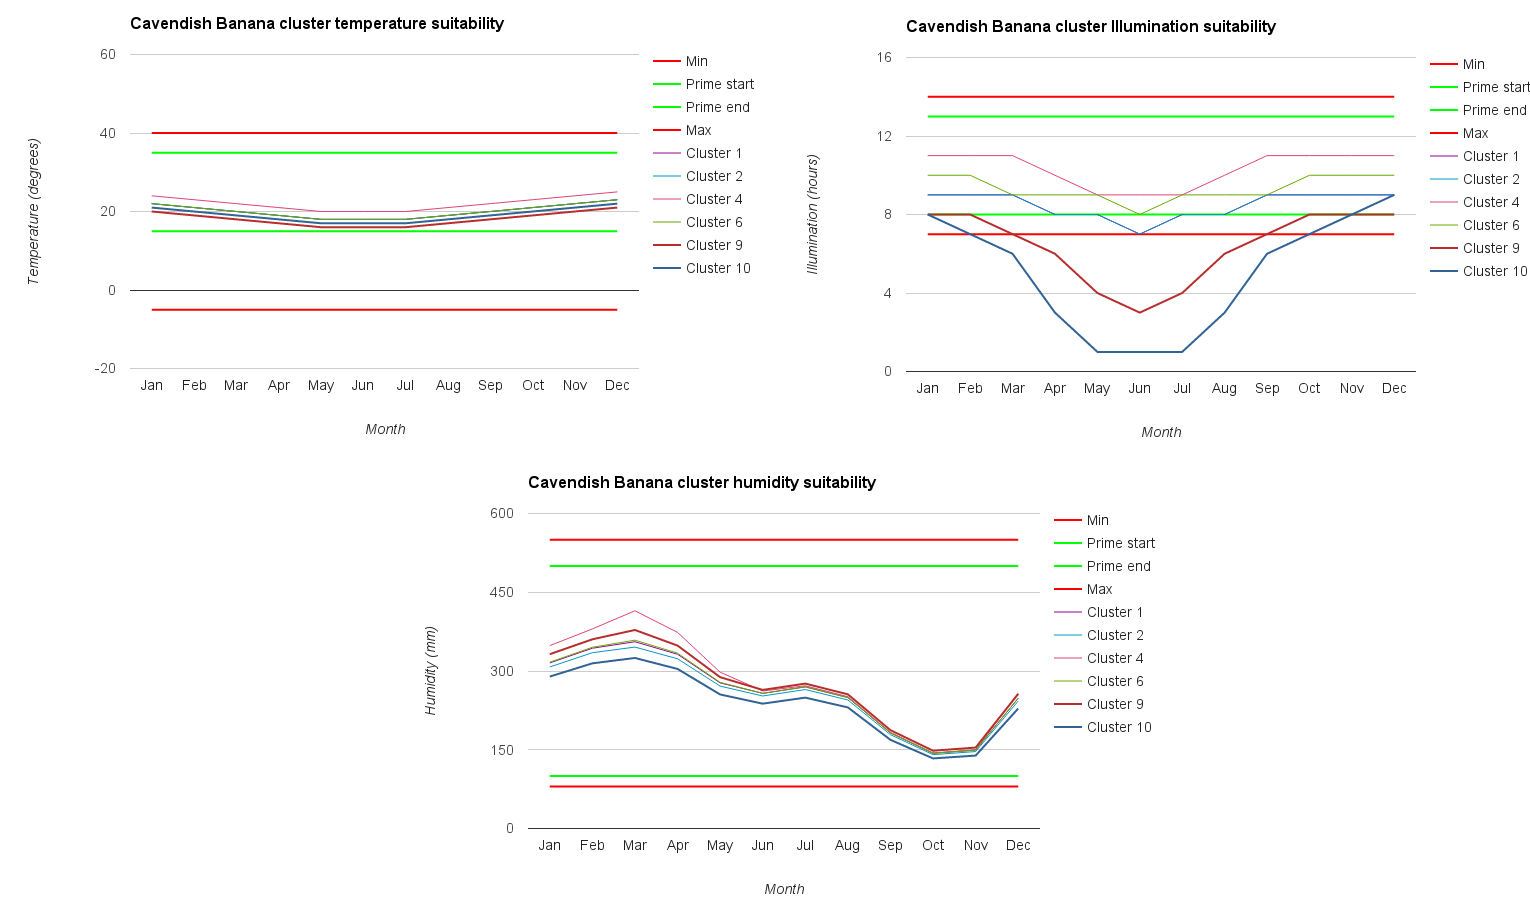
\includegraphics[height=\textheight-100pt,keepaspectratio]{cavendish_banana_suitability.png}
	\caption{ \textit{Tropical rainforest: Cavendish Banana suitability to clusters 1, 2, 4, 6, 9 and 10 in terms of soil moisture (top), illumination (middle) and temperature. The thick green lines and red lines delimit the species prime range and absolute limits, respectively.}}
	\label{fig:results_tropical_cavendish_banana_suitability}
\end{figure}

\begin{figure}[htb!]
\center
	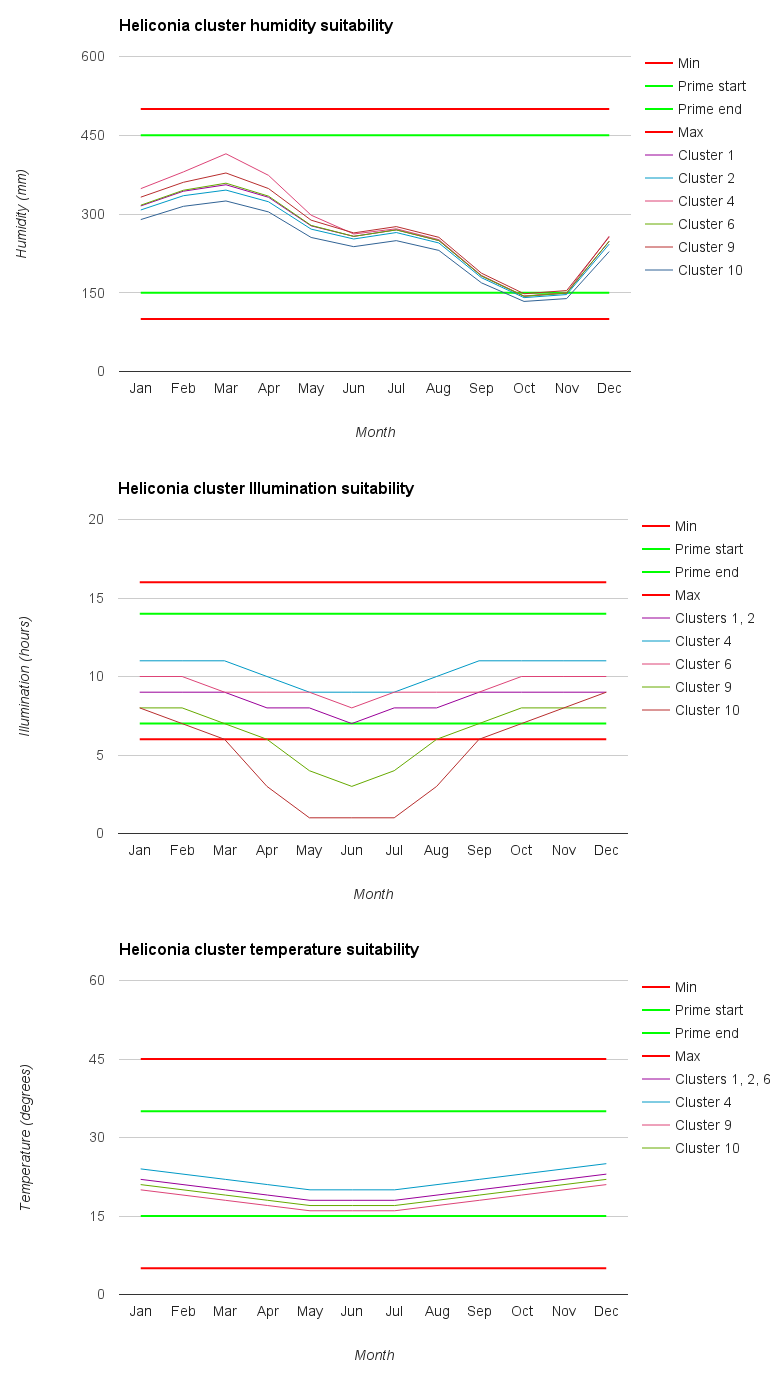
\includegraphics[height=\textheight-100pt,keepaspectratio]{heliconia_suitability.png}
	\caption{\textit{Tropical rainforest: Heliconia suitability to clusters 1, 2, 4, 6, 9 and 10 in terms of soil moisture (top), illumination (middle) and temperature. The thick green lines and red lines delimit the species prime range and absolute limits, respectively.}}
	\label{fig:results_tropical_heliconia_suitability}
\end{figure}

\begin{figure}[htb!]
\center
	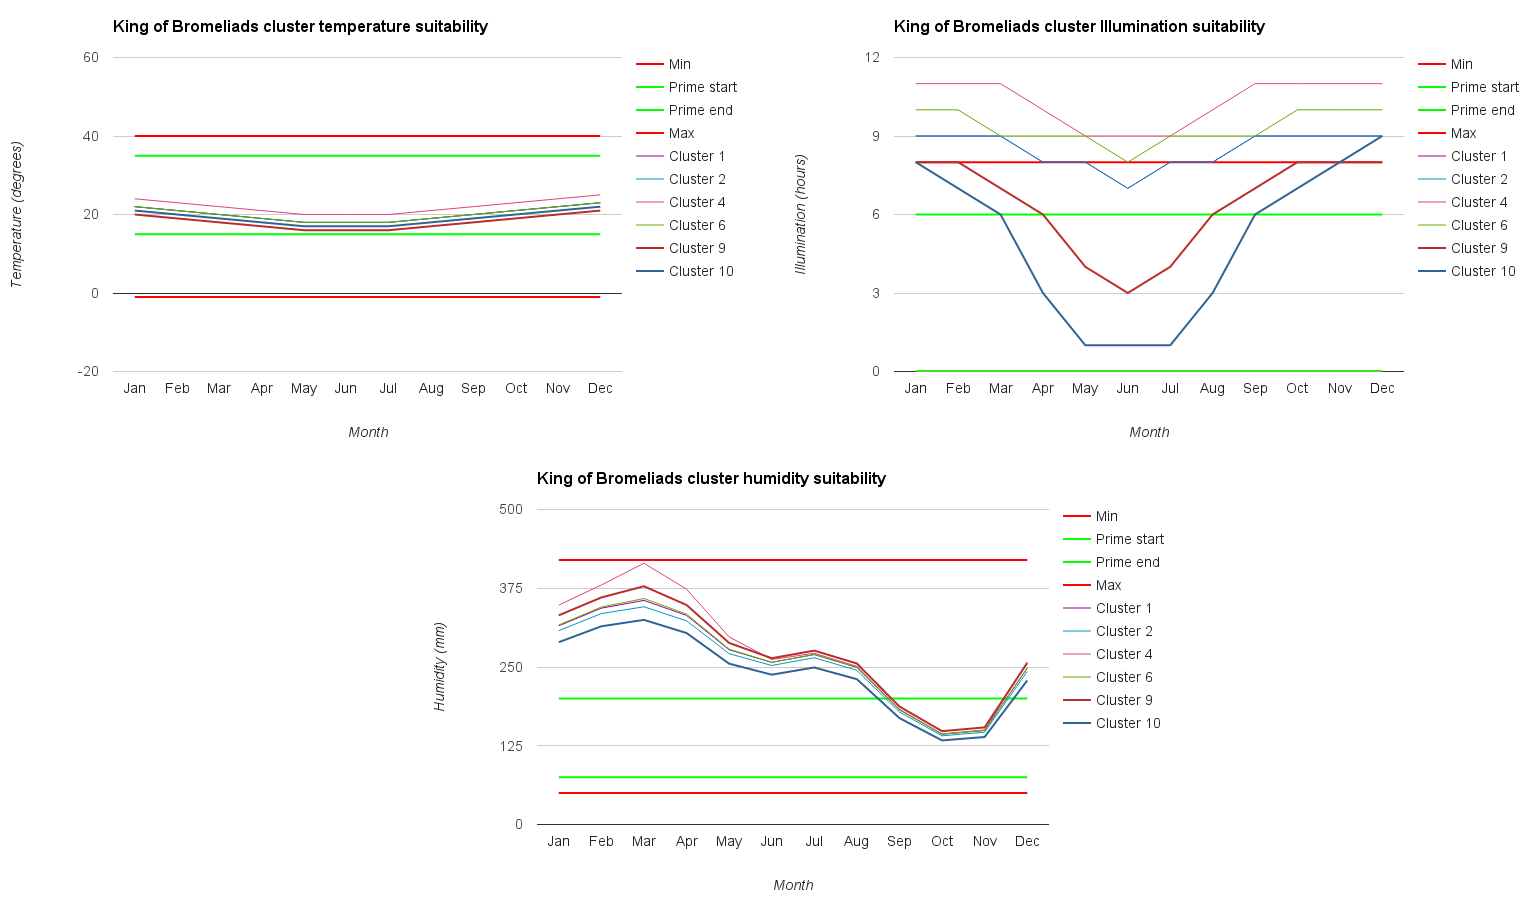
\includegraphics[height=\textheight-100pt,keepaspectratio]{king_of_bromeliads_suitability.png}
	\caption{ \textit{Tropical rainforest: King of Bromeliads suitability to clusters 1, 2, 4, 6, 9 and 10 iin terms of soil moisture (top), illumination (middle) and temperature. The thick green lines and red lines delimit the species prime range and absolute limits, respectively. Note that because the king of bromeliads is a shade-loving species, the minimum illumination line is not present as it is overlapped by the start of prime range line.}}
	\label{fig:results_tropical_king_of_bromeliads_suitability}
\end{figure}

\begin{figure}[htb!]
\center
	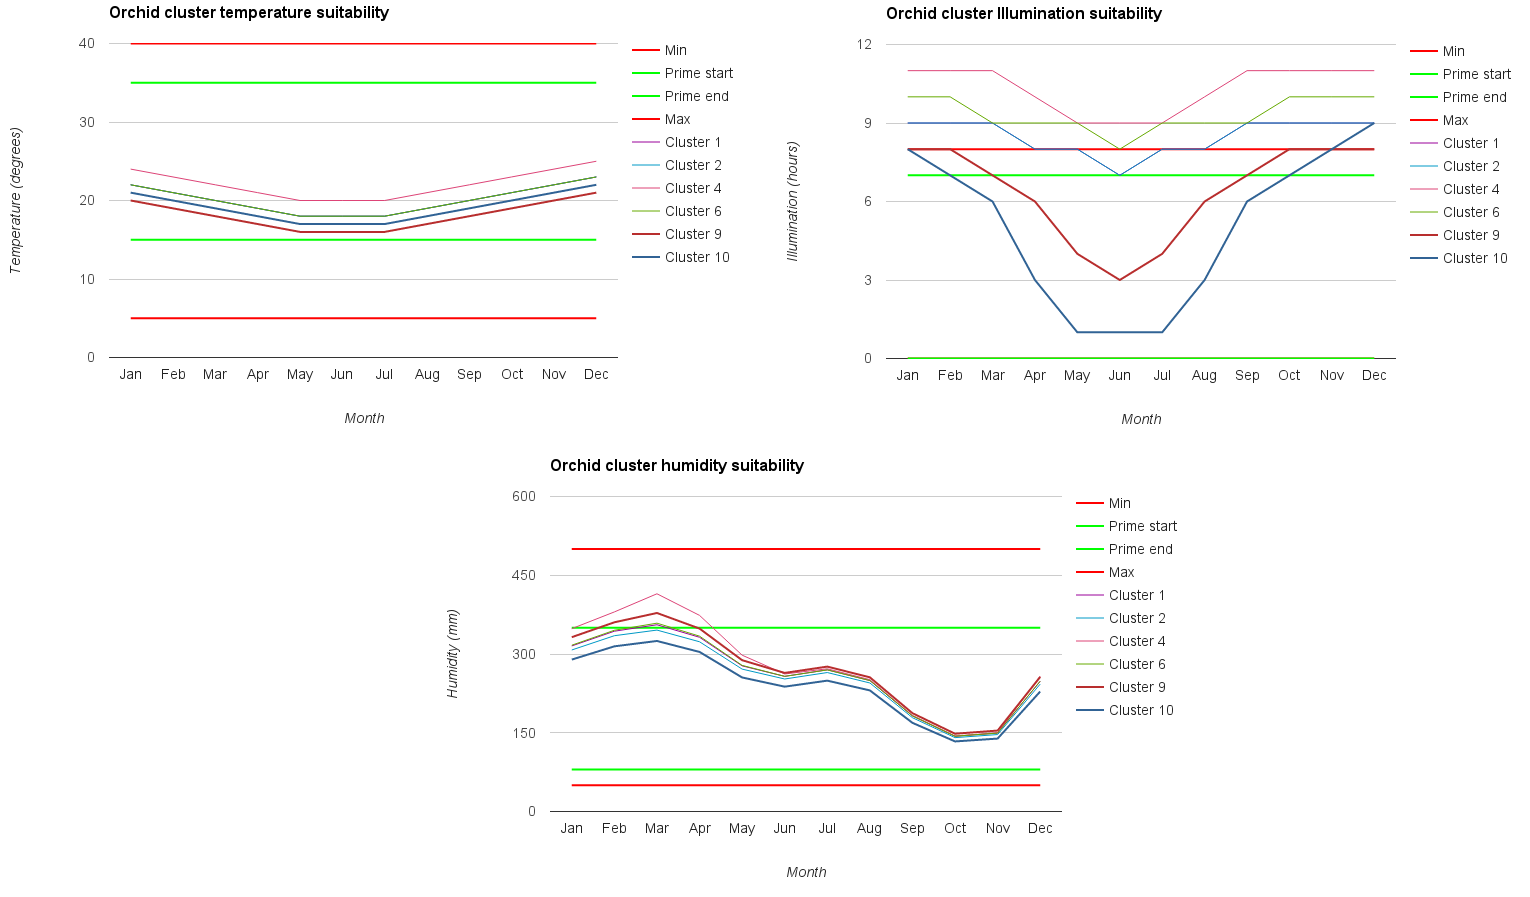
\includegraphics[height=\textheight-100pt,keepaspectratio]{orchid_suitability.png}
	\caption{ \textit{Tropical rainforest: Orchid suitability to clusters 1, 2, 4, 6, 9 and 10 in terms of soil moisture (top), illumination (middle) and temperature. The thick green lines and red lines delimit the species prime range and absolute limits, respectively. Note that because the king of bromeliads is a shade-loving specie, the minimum illumination line is not present as it is overlapped by the start of prime range line.}}
	\label{fig:results_tropical_orchid_suitability}
\end{figure}

\begin{table}[htb!]
  \centering
	    \begin{tabular}{|p{2cm}|p{2.5cm}|p{2.5cm}|p{2.5cm}|p{2.5cm}|p{2.5cm}|}
		\hline	
  	     & \textbf{Brazil Nut} & \textbf{Cavendish Banana} & \textbf{Heliconia} & \textbf{King of Bromeliads} & \textbf{Orchid} \\
  	    \hline	
		\textbf{Start of decline} & 
		15 & 
		20 & 
		25 &
		35 & 
		35 \\
		\hline
		\textbf{Max} & 
		25 &
		30 &
		40 &
		45 & 
		55 \\
		\hline
		\textbf{Cluster 1} & 
		\cellcolor{color_orange}22.3 &
		\cellcolor{color_orange}22.3 &
		\cellcolor{color_green}22.3 &
		\cellcolor{color_green}22.3 &
		\cellcolor{color_green}22.3 \\
		\hline
		\textbf{Cluster 2} & 
		\cellcolor{color_red}32.2 &
		\cellcolor{color_red}32.2 &
		\cellcolor{color_orange}32.2 &
		\cellcolor{color_green}32.2 &
		\cellcolor{color_green}32.2 \\
		\hline
		\textbf{Cluster 4} & 
		\cellcolor{color_green}2.9 & 
		\cellcolor{color_green}2.9 &
		\cellcolor{color_green}2.9 &
		\cellcolor{color_green}2.9 &
		\cellcolor{color_green}2.9 \\
		\hline
		\textbf{Cluster 6} & 
		\cellcolor{color_green}11.8 & 
		\cellcolor{color_green}11.8 &
		\cellcolor{color_green}11.8 &
		\cellcolor{color_green}11.8 &
		\cellcolor{color_green}11.8 \\
		\hline
		\textbf{Cluster 9} & 
		\cellcolor{color_green}14 & 
		\cellcolor{color_green}14 &
		\cellcolor{color_green}14 &
		\cellcolor{color_green}14 &
		\cellcolor{color_green}14 \\
		\hline
		\textbf{Cluster 10} & 
		\cellcolor{color_red}32.1 & 
		\cellcolor{color_red}32.1 &
		\cellcolor{color_orange}32.1 &
		\cellcolor{color_green}32.1 &
		\cellcolor{color_green}32.1 \\
		\hline
		\end{tabular}
		\caption{Tropical rainforest: Species suitability to clusters 1, 2, 4, 6, 9 and 10 in terms of slope, where: Green means the species is completely suited, orange means the species is negatively impacted by the slope, and red that the species is completely ill-suited. All values are in \textit{degrees}.}
	  \label{tab:results_tropical_species_slope_suitability}
\end{table}

Table \ref{tab:results_tropical_species_cluster_properties} summarizes the plant distributions generated by the ecosystem simulator for each cluster by stating the associated plant instance count, average, minimum and maximum size. We discuss each cluster separately below. \\

\paragraph{Cluster One}
Cluster one only permits Heliconia species to grow. As stated previously, \textit{Brazil Nut} and \textit{Cavendish Banana} plants are unable to grow in this cluster due to unsuitable illumination. \textit{King of Bromeliads} and \textit{Orchids} are also unable to grow as, without \textit{Brazil Nut} and \textit{Cavendish Banana} plants, these species lack the essential canopy shade necessary to grow. Although Heliconia thrives well in this cluster, because this species does not live long (it starts to decline after 3 years), it does not provide cover for shade-loving species long enough for them to develop and survive in the long term.

\paragraph{Cluster Two}

For the same reasons as for cluster one, all but Heliconia species are unable to grow in this cluster. However, as shown by its average size, this species fares poorly in this cluster, mostly because at 32 \textdegree, the clusters slope is outside the species optimal range.

\paragraph{Cluster Four}

Unlike clusters one and two, cluster four permits \textit{Brazil Nut} and \textit{Cavendish Banana} plants to grow which, in turn, permit shade-loving \textit{King of Bromeliads} and \textit{Orchids}. This cluster is close to optimal for all species and, as such, all species come close to reaching there maximum sizes. It covers 18\% of the terrain.

\paragraph{Cluster Six}

The distribution generated for cluster six is very similar to that of cluster four. With a bit less illumination and humidity available, however, the resource intensive \textit{Brazil Nut} and \textit{Cavendish Banana} thrive a bit less which, in turn, also provides fewer shade-loving plants.\\
Unlike other plant species, \textit{Heliconia} reaches a greater average size in this cluster compared to cluster five. Because this species has a short lifespan, the plant instances iteratively spawn and die. When they spawn, they are competing for resources against much more vigorous (large) plants and therefore struggle to get the resources necessary for there development. In this cluster the most vigorous plants (\textit{Brazil Nut} and \textit{Cavendish Banana}) survive less well and the competition for available resources is that much less intense, making it slightly easier for these plant species.\\

\begin{table}[htb!]
  \centering
	    \begin{tabular}{|p{2cm}|p{2cm}|p{2cm}|p{2cm}|p{2cm}|p{2cm}|}
		\hline	
		\textbf{Specie} & \textbf{Property} & \textbf{Cluster 1} & \textbf{Cluster 2} & \textbf{Cluster 4} & \textbf{Cluster 6} \\
		\hline
		% BRAZIL NUT 3
		\multirow{4}{*}{\textbf{Brazil Nut}} & 
						\multicolumn{1}{l|}{Count} & 
						\multicolumn{1}{l|}{0} & 
						\multicolumn{1}{l|}{0} &
						\multicolumn{1}{l|}{324} & 
						\multicolumn{1}{l|}{342} \\\cline{2-6} &
						\multicolumn{1}{l|}{Min height (cm)} & 
						\multicolumn{1}{l|}{-} & 
						\multicolumn{1}{l|}{-} &
						\multicolumn{1}{l|}{11} & 
						\multicolumn{1}{l|}{19} \\\cline{2-6} &
						\multicolumn{1}{l|}{Max height (cm)} & 
						\multicolumn{1}{l|}{-} & 
						\multicolumn{1}{l|}{-} &
						\multicolumn{1}{l|}{1879} & 
						\multicolumn{1}{l|}{1984} \\\cline{2-6} &
						\multicolumn{1}{l|}{Avg height (cm)} & 
						\multicolumn{1}{l|}{-} & 
						\multicolumn{1}{l|}{-} &
						\multicolumn{1}{l|}{396} & 
						\multicolumn{1}{l|}{357} \\\cline{2-6}
		\hline       
		% Cavendish Banana 5
		\multirow{4}{*}{\textbf{CB}} & 
						\multicolumn{1}{l|}{Count} & 
						\multicolumn{1}{l|}{0} & 
						\multicolumn{1}{l|}{0} &
						\multicolumn{1}{l|}{371} & 
						\multicolumn{1}{l|}{408} \\\cline{2-6} &
						\multicolumn{1}{l|}{Min height (cm)} & 
						\multicolumn{1}{l|}{-} & 
						\multicolumn{1}{l|}{-} &
						\multicolumn{1}{l|}{2} & 
						\multicolumn{1}{l|}{4} \\\cline{2-6} &
						\multicolumn{1}{l|}{Max height (cm)} & 
						\multicolumn{1}{l|}{-} & 
						\multicolumn{1}{l|}{-} &
						\multicolumn{1}{l|}{215} & 
						\multicolumn{1}{l|}{215} \\\cline{2-6} &
						\multicolumn{1}{l|}{Avg height (cm)} & 
						\multicolumn{1}{l|}{-} & 
						\multicolumn{1}{l|}{-} &
						\multicolumn{1}{l|}{70} & 
						\multicolumn{1}{l|}{64} \\\cline{2-6}
		\hline      
		%Heliconia 2 
		\multirow{4}{*}{\textbf{Heliconia}} & 
						\multicolumn{1}{l|}{Count} & 
						\multicolumn{1}{l|}{625} & 
						\multicolumn{1}{l|}{1456} &
						\multicolumn{1}{l|}{766} & 
						\multicolumn{1}{l|}{793} \\\cline{2-6} &
						\multicolumn{1}{l|}{Min height (cm)} & 
						\multicolumn{1}{l|}{5} & 
						\multicolumn{1}{l|}{1} &
						\multicolumn{1}{l|}{5} & 
						\multicolumn{1}{l|}{9} \\\cline{2-6} &
						\multicolumn{1}{l|}{Max height (cm)} & 
						\multicolumn{1}{l|}{297} & 
						\multicolumn{1}{l|}{22} &
						\multicolumn{1}{l|}{298} & 
						\multicolumn{1}{l|}{298} \\\cline{2-6} &
						\multicolumn{1}{l|}{Avg height (cm)} & 
						\multicolumn{1}{l|}{132.8} & 
						\multicolumn{1}{l|}{10.2} &
						\multicolumn{1}{l|}{136.5} & 
						\multicolumn{1}{l|}{140} \\\cline{2-6}
		\hline      
		% King of Bromeliads 1
		\multirow{4}{*}{\textbf{KOB}} & 
						\multicolumn{1}{l|}{Count} & 
						\multicolumn{1}{l|}{0} & 
						\multicolumn{1}{l|}{0} &
						\multicolumn{1}{l|}{612} & 
						\multicolumn{1}{l|}{281} \\\cline{2-6} &
						\multicolumn{1}{l|}{Min height (cm)} & 
						\multicolumn{1}{l|}{-} & 
						\multicolumn{1}{l|}{-} &
						\multicolumn{1}{l|}{6} & 
						\multicolumn{1}{l|}{16} \\\cline{2-6} &
						\multicolumn{1}{l|}{Max height (cm)} & 
						\multicolumn{1}{l|}{-} & 
						\multicolumn{1}{l|}{-} &
						\multicolumn{1}{l|}{86} & 
						\multicolumn{1}{l|}{78} \\\cline{2-6} &
						\multicolumn{1}{l|}{Avg height (cm)} & 
						\multicolumn{1}{l|}{-} & 
						\multicolumn{1}{l|}{-} &
						\multicolumn{1}{l|}{41} & 
						\multicolumn{1}{l|}{38} \\\cline{2-6}
		\hline     
		% Orchid 4
		\multirow{4}{*}{\textbf{Orchid}} & 
						\multicolumn{1}{l|}{Count} & 
						\multicolumn{1}{l|}{0} & 
						\multicolumn{1}{l|}{0} &
						\multicolumn{1}{l|}{557} & 
						\multicolumn{1}{l|}{260} \\\cline{2-6} &
						\multicolumn{1}{l|}{Min height (cm)} & 
						\multicolumn{1}{l|}{-} & 
						\multicolumn{1}{l|}{-} &
						\multicolumn{1}{l|}{1} & 
						\multicolumn{1}{l|}{2} \\\cline{2-6} &
						\multicolumn{1}{l|}{Max height (cm)} & 
						\multicolumn{1}{l|}{-} & 
						\multicolumn{1}{l|}{-} &
						\multicolumn{1}{l|}{36} & 
						\multicolumn{1}{l|}{45} \\\cline{2-6} &
						\multicolumn{1}{l|}{Avg height (cm)} & 
						\multicolumn{1}{l|}{-} & 
						\multicolumn{1}{l|}{-} &
						\multicolumn{1}{l|}{8.5} & 
						\multicolumn{1}{l|}{6.2} \\\cline{2-6}
		\hline                                                       
		\end{tabular}
	\caption{Tropical rainforest: Vegetation content of the hundred by hundred metre simulation window for each cluster. CB and KOB represent species Cavendish Banana and King of Bromeliads, respectively.}
	\label{tab:results_tropical_species_cluster_properties}	
\end{table}

